% Provenance (never printed): old terminale S material on absolute dating (the
% decay law recalled, the closed system, the rubidium-strontium isochron) and on
% the history of the age of the Earth (cooling, salt, sediments, then radioactivity,
% meteorites and 4.55 billion years). Owner (Sync 0/1): closed system, isochron,
% age of the Earth (as a defined notion). The decay law, the half-life and the
% dating equation are the physics books' (recalled); relative dating, absolute
% age, superposition, cross-cutting relationships and the eras are Book 1 g7's
% (recalled); the oldest zircons and the Acasta gneiss are g12.01's (quoted).
% Varden Hills granite 310 Ma and schist 480 Ma from figdata/shared/region.py;
% their isotope ratios are exercise data (figdata/grade-12/isochrons.py).
\chapter{التأريخ الإشعاعي وعمر الأرض}\label{ch:g12:age-of-the-earth}

في عام 1862 حسب الفيزيائي وليام طومسون، الذي صار فيما بعد اللورد كلفن، \omterm{def:g12:age-of-the-earth:age}{عمر
الأرض} من طريقة تبردها. فقد افترض أنها تكوّنت منصهرة وظلت
تفقد حرارتها منذ ذلك الحين، وتساءل كم يلزم من الوقت لكي ينخفض
تدرج درجة الحرارة قرب السطح إلى قيمته الحالية. وكان
جوابه 96 مليون سنة، في مكان ما بين 20 و400
مليون؛ وبحلول عام 1897 كان قد ضيّقه إلى ما بين 20 و40 مليونًا.
ورأى الجيولوجيون ذلك أقصر بكثير من التاريخ الذي يقرؤونه في الصخور.
وجاء الجواب من النشاط الإشعاعي، الذي لم يكن كلفن يعرفه.
% ledger: holmes13:estimates, england:kelvin (Book 3 row)

\begin{omfigure}
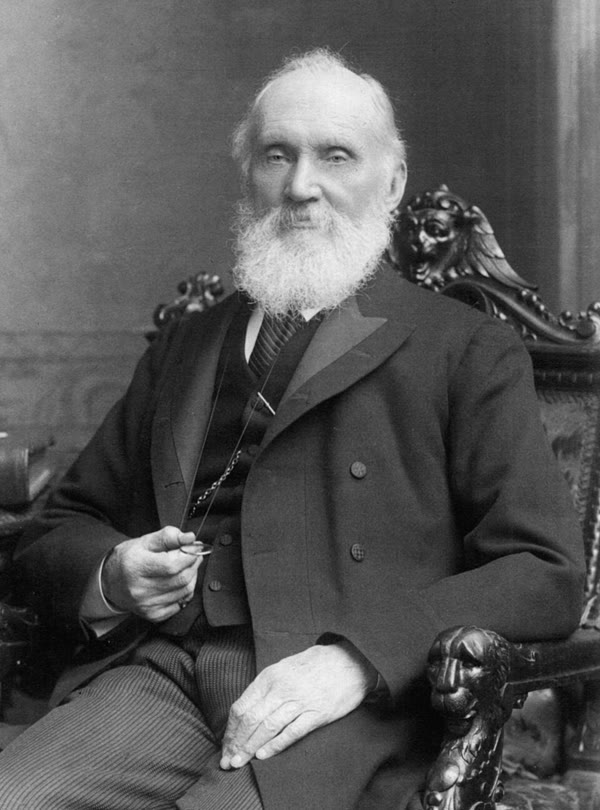
\includegraphics[height=5.2cm]{images/book2/g12-kelvin-1906.jpg}

{\small وليام طومسون، اللورد كلفن، في عام 1906. الصورة: راسل وأبناؤه،
لندن (مكتبات مؤسسة سميثسونيان، دون قيود معروفة لحقوق النشر).}
\end{omfigure}
% ledger: photo:g12-kelvin

\begin{recall}
يرتّب التأريخ النسبي الصخور والأحداث؛ أما العمر المطلق فعدد
من السنين (الكتاب 1، الصف 7). والنظير المشع، أي النظير الأم، يتفكك إلى
نظير وليد عشوائيًا: فعدد $N$ من ذرات الأم الباقية يتناقص وفق
$N = N_0\,e^{-\lambda t}$، حيث $\lambda$ ثابت التفكك، وينتصف
كل عمر نصف $T = \ln 2/\lambda$ (كتب الفيزياء). وأقدم المعادن
المعروفة، حبيبات زركون من غرب أستراليا، عمرها 4.4 مليار سنة
(\cref{ch:g12:continental-crust}). والأرض تفقد أيضًا حرارة يظل النشاط الإشعاعي
يصنعها، ووشاحها يتحرك \omterm{def:g12:internal-heat:convection}{بالحمل الحراري} (\cref{ch:g12:internal-heat}).
\end{recall}
% ledger: wilde01:zircon

\section{تاريخ التقديرات}

قبل النشاط الإشعاعي، كان كل تقدير \omterm{def:g12:age-of-the-earth:age}{لعمر الأرض} يستند إلى عملية
يُفترض أن معدلها معروف.

\begin{center}
\small
\begin{tabular}{|p{0.19\linewidth}|p{0.42\linewidth}|p{0.25\linewidth}|}
\hline
من، ومتى & الطريقة وما تفترضه & التقدير \\
\hline
فيليبس، 1860 & سمك الطبقات الرسوبية مقسومًا على معدل للترسيب؛ تفترض معدلًا ثابتًا & من 38 إلى 96 مليون سنة \\
كلفن، 1862 & تبرد أرض منصهرة بالتوصيل وحده، دون أي مصدر للحرارة في داخلها & من 20 إلى 400 مليون سنة \\
ج.\,ه.~داروين & الزمن منذ انفصال القمر عن الأرض، من تباطؤ حركتيهما بفعل المد والجزر & 56 مليون سنة على الأقل \\
جولي، 1899 & الملح الذي تحمله الأنهار إلى البحر، مقسومًا على الإمداد السنوي؛ تفترض إمدادًا ثابتًا وعدم إزالة أي ملح & من 80 إلى 100 مليون سنة \\
\hline
\end{tabular}
\end{center}
% ledger: holmes13:estimates

\begin{history}[حرارة كلفن المفقودة]
في عام 1903 بيّن بيير كوري وألبير لابورد أن الراديوم يطلق حرارة،
وسرعان ما رأى عدد من العلماء أن هذه الحرارة تنقض استنتاج
كلفن. وبعد عام، ذكّر إرنست رذرفورد كلفن، في محاضرة كان كلفن بين
حاضريها، بأنه حدّ \omterm{def:g12:age-of-the-earth:age}{عمر الأرض}
«ما لم يُكتشف مصدر جديد للحرارة». وبدا أن النشاط الإشعاعي هو
ذلك المصدر. ومع ذلك لم يكن هذا خطأ كلفن الأكبر: فأكثر ما يطيل تبرد الأرض
هو \omterm{def:g12:internal-heat:convection}{الحمل الحراري في الوشاح}، الذي يُبقي الوشاح العلوي ساخنًا والتدرج في
القشرة مرتفعًا مدة أطول بكثير مما يفعله التوصيل وحده.
\end{history}
% ledger: england:kelvin (Book 3 row)

وقدّم النشاط الإشعاعي أيضًا ساعة. ففي عام 1907 بيّن برترام بولتوود أن
معادن اليورانيوم المتساوية العمر تحوي القدر نفسه من الرصاص لكل غرام
من اليورانيوم: فالرصاص يصنعه اليورانيوم. وبحلول عام 1913 استطاع آرثر هولمز أن
يكتب أن أقدم الصخور المؤرَّخة عمرها \num{1600} مليون سنة، وفي
عام 1927 جعل \omterm{def:g12:age-of-the-earth:age}{عمر الأرض} بين 1.6 و3.0 مليار سنة. وفي عام 1956 قاس كلير
باترسون 4.55 مليار سنة. والقيمة المعتمدة اليوم 4.54 مليار سنة،
بدقة واحد في المئة.
% ledger: holmes13:estimates, holmes27:age, patterson56:table, usgs:age-earth (Book 1 row)

\begin{omfigure}
\begin{tikzpicture}
\begin{axis}[omrecord, width=0.78\linewidth, height=6.2cm, ymode=log, xmin=1840, xmax=2040,
  ymin=1e7, ymax=2e10, xlabel={\foreignlanguage{arabic}{سنة التقدير}}, ylabel={\foreignlanguage{arabic}{عمر الأرض المقدَّر بالسنين}},
  xtick={1850,1875,...,2025}, x tick label style={/pgf/number format/.cd, set thousands separator={}},
  ytick={1e7,1e8,1e9,1e10}, ymajorgrids=true, xmajorgrids=false]
% computed in figdata/grade-12/isochrons.py; ledger: holmes13:estimates, holmes27:age, patterson56:table, usgs:age-earth (Book 1 row)
\addplot[omDef, only marks, mark=*, mark size=1.8pt, error bars/.cd, y dir=both, y explicit]
  table[x=year, y=mid, y error minus expr=\thisrow{mid}-\thisrow{lo}, y error plus expr=\thisrow{hi}-\thisrow{mid}]
  {figdata/out/grade-12-isochrons-history.dat};
\addplot[omThm, densely dashed, domain=1840:2040, samples=2] {4.54e9};
\coordinate (k62) at (axis cs:1862,2.4e8);
\coordinate (k97) at (axis cs:1897,2.8e7);
\coordinate (jol) at (axis cs:1899,1e8);
\coordinate (h11) at (axis cs:1919,1.3e9);
\coordinate (pat) at (axis cs:1956,4.55e9);
\coordinate (now) at (axis cs:1845,4.54e9);
\end{axis}
\node[font=\scriptsize, anchor=west] at ([xshift=4pt]k62) {\foreignlanguage{arabic}{كلفن 1862}};
\node[font=\scriptsize, anchor=east] at ([xshift=-4pt]k97) {\foreignlanguage{arabic}{كلفن 1897}};
\node[font=\scriptsize, anchor=west] at ([xshift=4pt]jol) {جولي};
\node[font=\scriptsize, anchor=north] at (h11) {هولمز};
\node[font=\scriptsize, anchor=north west] at ([xshift=2pt, yshift=-3pt]pat) {باترسون};
\node[font=\scriptsize, text=omThm, anchor=south west] at (now) {\foreignlanguage{arabic}{اليوم، 4.54 مليار سنة}};
\end{tikzpicture}

{\small تقديرات \omterm{def:g12:age-of-the-earth:age}{عمر الأرض} بدلالة السنة التي وُضعت فيها، على
مقياس لوغاريتمي؛ وتمتد القضبان على المدى الذي أعطاه كل مؤلف. ونقطة هولمز لعام 1913
هي عمر أقدم الصخور المؤرَّخة حينئذ، أي حد أدنى. المصادر: هولمز
(1913، 1927)؛ باترسون (1956)؛ هيئة المسح الجيولوجي الأمريكية.}
\end{omfigure}

\section{ساعة إشعاعية}

لا تعمل الساعة الإشعاعية إلا إذا لم يُضَف إليها شيء ولم يُنتزع منها
شيء منذ أن بدأت.

\begin{definition}[النظام المغلق]\label{def:g12:age-of-the-earth:closed-system}
يكون الصخر أو المعدن \emph{نظامًا مغلقًا}\index{نظام مغلق} بالنسبة إلى
نظير أم ونظيره الوليد إذا لم تدخله ولم تخرج منه، منذ لحظة بدء ساعته،
أي ذرة من الأم أو من الوليد، إلا ما كان
بتفكك الأم إلى الوليد.
\end{definition}
% ledger: tulane:radiometric

تبدأ ساعة المعدن حين يتبلور من صهارة، أو بدقة
أكبر حين يبرد بما يكفي لتكف الذرات عن الدخول إليه والخروج
منه. والتسخين، أو مائع
ساخن، أو التجوية، قد تفتح النظام من جديد، فيكون العمر المقيس حينئذ
خاطئًا، أو يؤرّخ ذلك الحدث اللاحق.
% ledger: tulane:radiometric

عدّ الذرات الوليدة في \omterm{def:g12:age-of-the-earth:closed-system}{نظام مغلق} يعطي العمر، بشرط أن
نعرف كم كان منها في البداية. وعادة لا نعرف ذلك. فالروبيديوم-87
يتفكك إلى السترونتيوم-87، لكن كل معدن أخذ أيضًا شيئًا من السترونتيوم-87
حين تكوّن. وطريقة \omterm{def:g12:age-of-the-earth:isochron}{خط تساوي العمر} تتغلب على ذلك بقياس عدة
معادن من صخر واحد.

\section{خط تساوي العمر}

للسترونتيوم نظير، السترونتيوم-86، مستقر ولا يصنعه أي
تفكك: ففي \omterm{def:g12:age-of-the-earth:closed-system}{النظام المغلق} يبقى عدده ثابتًا، ويصلح
مقياسًا مرجعيًا. والنسبتان النظيريتان $^{87}\mathrm{Sr}/^{86}\mathrm{Sr}$
و$^{87}\mathrm{Rb}/^{86}\mathrm{Sr}$ هما ما يقيسه مطياف الكتلة.

\begin{theorem}[معادلة خط تساوي العمر]\label{thm:g12:age-of-the-earth:isochron}
في معدن ظل \omterm{def:g12:age-of-the-earth:closed-system}{نظامًا مغلقًا} مدة $t$،
\[
  \left(\frac{^{87}\mathrm{Sr}}{^{86}\mathrm{Sr}}\right)_{\text{الآن}}
  = \left(\frac{^{87}\mathrm{Sr}}{^{86}\mathrm{Sr}}\right)_{0}
  + \left(\frac{^{87}\mathrm{Rb}}{^{86}\mathrm{Sr}}\right)_{\text{الآن}}
  \left(e^{\lambda t} - 1\right),
\]
حيث يدل الدليل 0 على القيمة عند بدء الساعة، و$\lambda$
ثابت تفكك الروبيديوم-87.
\end{theorem}

\begin{proof}
ليكن $P$ عدد ذرات الروبيديوم-87 الآن و$P_0$ عددها عند بدء
الساعة. بحسب قانون التفكك $P = P_0\,e^{-\lambda t}$، إذن $P_0 = P\,e^{\lambda t}$،
وعدد الذرات التي تفككت هو $P_0 - P = P\,(e^{\lambda t}-1)$.
وفي \omterm{def:g12:age-of-the-earth:closed-system}{النظام المغلق} صارت كل منها ذرة واحدة من السترونتيوم-87، تُضاف
إلى الذرات $D_0$ الموجودة في البداية: $D = D_0 + P\,(e^{\lambda
t}-1)$. وبالقسمة على عدد ذرات السترونتيوم-86، الذي لم يتغير،
نحصل على المعادلة.
\end{proof}
% ledger: tulane:radiometric

تبلورت معادن الغرانيت من صهارة واحدة، فبدأت كلها
بالنسبة نفسها $(^{87}\mathrm{Sr}/^{86}\mathrm{Sr})_0$. لكنها أخذت
كميات مختلفة جدًا من الروبيديوم. وبما أنها كلها تشترك في $t$ نفسه وفي النسبة الابتدائية نفسها،
فالمعادلة تقول إن نقاطها تقع على خط مستقيم واحد.

\begin{definition}[خط تساوي العمر]\label{def:g12:age-of-the-earth:isochron}
\emph{خط تساوي العمر}\index{خط تساوي العمر} هو الخط المستقيم الذي تقع عليه
نقاط معادن أو صخور تكوّنت في الوقت نفسه من المصدر
نفسه وظلت أنظمة مغلقة منذ ذلك الحين، حين تُرسم نسبة النظير الوليد إلى
النظير المستقر بدلالة نسبة النظير الأم إلى النظير المستقر. ويعطي
ميله عمرها، وتعطي النقطة التي يلاقي فيها المحور الرأسي
نسبتها الابتدائية.
\end{definition}
% ledger: tulane:radiometric

\begin{proposition}[العمر من الميل]\label{prop:g12:age-of-the-earth:slope}
إذا كان ميل \omterm{def:g12:age-of-the-earth:isochron}{خط تساوي العمر} $m$، فالعمر هو
\[
  t = \frac{\ln(1+m)}{\lambda}.
\]
\end{proposition}

\begin{proof}
بالمقارنة مع معادلة \omterm{def:g12:age-of-the-earth:isochron}{خط تساوي العمر}، $m = e^{\lambda t} - 1$، إذن
$e^{\lambda t} = 1 + m$، و$\lambda t = \ln(1+m)$، و$t = \ln(1+m)/\lambda$.
\end{proof}

للروبيديوم-87، $\lambda = \num{1.3972e-11}$ في السنة، أي عمر نصف قدره
$\ln 2/\lambda \approx 49.6$ مليار سنة: أكثر من عشرة أضعاف \omterm{def:g12:age-of-the-earth:age}{عمر
الأرض}.
% ledger: villa22:rb87

\begin{method}[تأريخ صخر بخط تساوي العمر]\label{met:g12:age-of-the-earth:isochron}
\begin{enumerate}
  \item افصل عدة معادن من الصخر (أو خذ منه عدة
        عينات) تختلف كميات الروبيديوم فيها.
  \item قِس في كل منها النسبتين $^{87}\mathrm{Rb}/^{86}\mathrm{Sr}$ ($x$)
        و$^{87}\mathrm{Sr}/^{86}\mathrm{Sr}$ ($y$).
  \item ارسم $y$ بدلالة $x$ وتحقق من أن النقاط تقع على خط
        مستقيم: فإن خرجت منها نقطة، لم تكن تلك العينة \omterm{def:g12:age-of-the-earth:closed-system}{نظامًا مغلقًا}.
  \item خذ ميل الخط $m$، واحسب $t = \ln(1+m)/\lambda$.
  \item اقرأ النسبة الابتدائية حيث يلاقي الخط المحور الرأسي.
\end{enumerate}
\end{method}

\begin{example}[غرانيت فاردن]\label{ex:g12:age-of-the-earth:varden}
يعطي غرانيت تلال فاردن، المنطقة المتخيَّلة في هذه السلسلة، هذه
النسب (بيانات تمرين):
\begin{center}
\small
\begin{tabular}{|l|c|c|}
\hline
العينة & $^{87}\mathrm{Rb}/^{86}\mathrm{Sr}$ & $^{87}\mathrm{Sr}/^{86}\mathrm{Sr}$ \\
\hline
بلاجيوكليز & 0.35 & 0.70952 \\
هورنبلند  & 1.20 & 0.71321 \\
الصخر الكلي  & 3.10 & 0.72146 \\
فلسبار البوتاسيوم  & 6.40 & 0.73578 \\
بيوتيت     & 24.0 & 0.81218 \\
\hline
\end{tabular}
\end{center}
عبر البلاجيوكليز والبيوتيت، يكون الميل
$m = (0.81218 - 0.70952)/(24.0 - 0.35) \approx 0.004341$. إذن
$t = \ln(1.004341)/\num{1.3972e-11} \approx \num{3.10e8}$ سنة:
فعمر الغرانيت 310 ملايين سنة. ويلاقي الخط المحور الرأسي عند
$0.70952 - 0.35 \times 0.004341 \approx 0.7080$، وهي النسبة الابتدائية.
\end{example}
% values: granite_age_Ma 310.0, granite_intercept 0.70800 (isochrons.py)

\begin{omfigure}
\begin{tikzpicture}
\begin{axis}[omrecord, width=0.7\linewidth, height=6cm, xmin=0, xmax=26, ymin=0.695, ymax=0.82, ytick={0.70,0.72,...,0.82},
  xlabel={$^{87}\mathrm{Rb}/^{86}\mathrm{Sr}$}, ylabel={$^{87}\mathrm{Sr}/^{86}\mathrm{Sr}$},
  y tick label style={/pgf/number format/.cd, fixed, fixed zerofill, precision=2}]
% computed in figdata/grade-12/isochrons.py (exercise data, Varden granite 310 Ma); ledger: villa22:rb87
\addplot[omDef, line width=0.9pt] table[x=x, y=y] {figdata/out/grade-12-isochrons-graniteln.dat};
\addplot[omThm, only marks, mark=*, mark size=2pt] table[x=rbsr, y=srsr] {figdata/out/grade-12-isochrons-granite.dat};
\addplot[black!60, densely dotted, domain=0:26, samples=2] {0.7080};
\coordinate (pl) at (axis cs:0.35,0.70952);
\coordinate (hb) at (axis cs:1.2,0.71321);
\coordinate (wr) at (axis cs:3.1,0.72146);
\coordinate (kf) at (axis cs:6.4,0.73578);
\coordinate (bt) at (axis cs:24,0.81218);
\coordinate (sl) at (axis cs:12,0.762);
\coordinate (in) at (axis cs:9,0.7082);
\coordinate (plhb) at (axis cs:0.6,0.737);
\coordinate (plhbpt) at (axis cs:0.9,0.7125);
\end{axis}
\node[font=\scriptsize, anchor=north west] at ([xshift=1pt]wr) {الصخر الكلي};
\node[font=\scriptsize, anchor=north west] at ([xshift=1pt]kf) {فلسبار البوتاسيوم};
\node[font=\scriptsize, anchor=east] at ([xshift=-3pt]bt) {بيوتيت};
\node[font=\scriptsize, anchor=south west, align=left, inner sep=1pt] (plhblab) at (plhb) {بلاجيوكليز\\وهورنبلند};
\draw[black!60, line width=0.4pt] (plhblab.south) -- (plhbpt);
\node[font=\scriptsize, text=omDef, anchor=south east] at (sl) {\foreignlanguage{arabic}{الميل $0.004341$: 310 ملايين سنة}};
\node[font=\scriptsize, text=black!70, anchor=south west] at (in) {\foreignlanguage{arabic}{النسبة الابتدائية 0.7080، عند الزمن 0}};
\end{tikzpicture}

{\small \omterm{def:g12:age-of-the-earth:isochron}{خط تساوي العمر} بالروبيديوم--السترونتيوم لغرانيت فاردن (بيانات
تمرين). حين تكوّن الغرانيت، كانت معادنه كلها على الخط الأفقي
المنقط؛ ومنذ ذلك الحين ارتفع كل منها بالتناسب مع ما فيه من الروبيديوم،
وهي الآن على الخط المتصل.}
\end{omfigure}

\begin{inthelab}[وزن الذرات]
تُقاس النسب بمطياف الكتلة. فتُذاب بضعة ملّيغرامات من
المعدن في حمض، ويُفصل السترونتيوم عن
الروبيديوم كيميائيًا، لأن النظيرين اللذين كتلتهما 87 كانا سيُعدّان
معًا لولا ذلك. ثم يوضع السترونتيوم على فتيل معدني ويُسخَّن
في الفراغ، فيطلق أيونات؛ ويسرّعها مجال كهربائي ويحني مغناطيسٌ
مساراتها، والأيونات الأخف أكثر انحناء من الأثقل، فيبلغ كل
نظير مجمِّعه الخاص. وتعطي تياراتها النسب.
\end{inthelab}

\begin{omfigure}
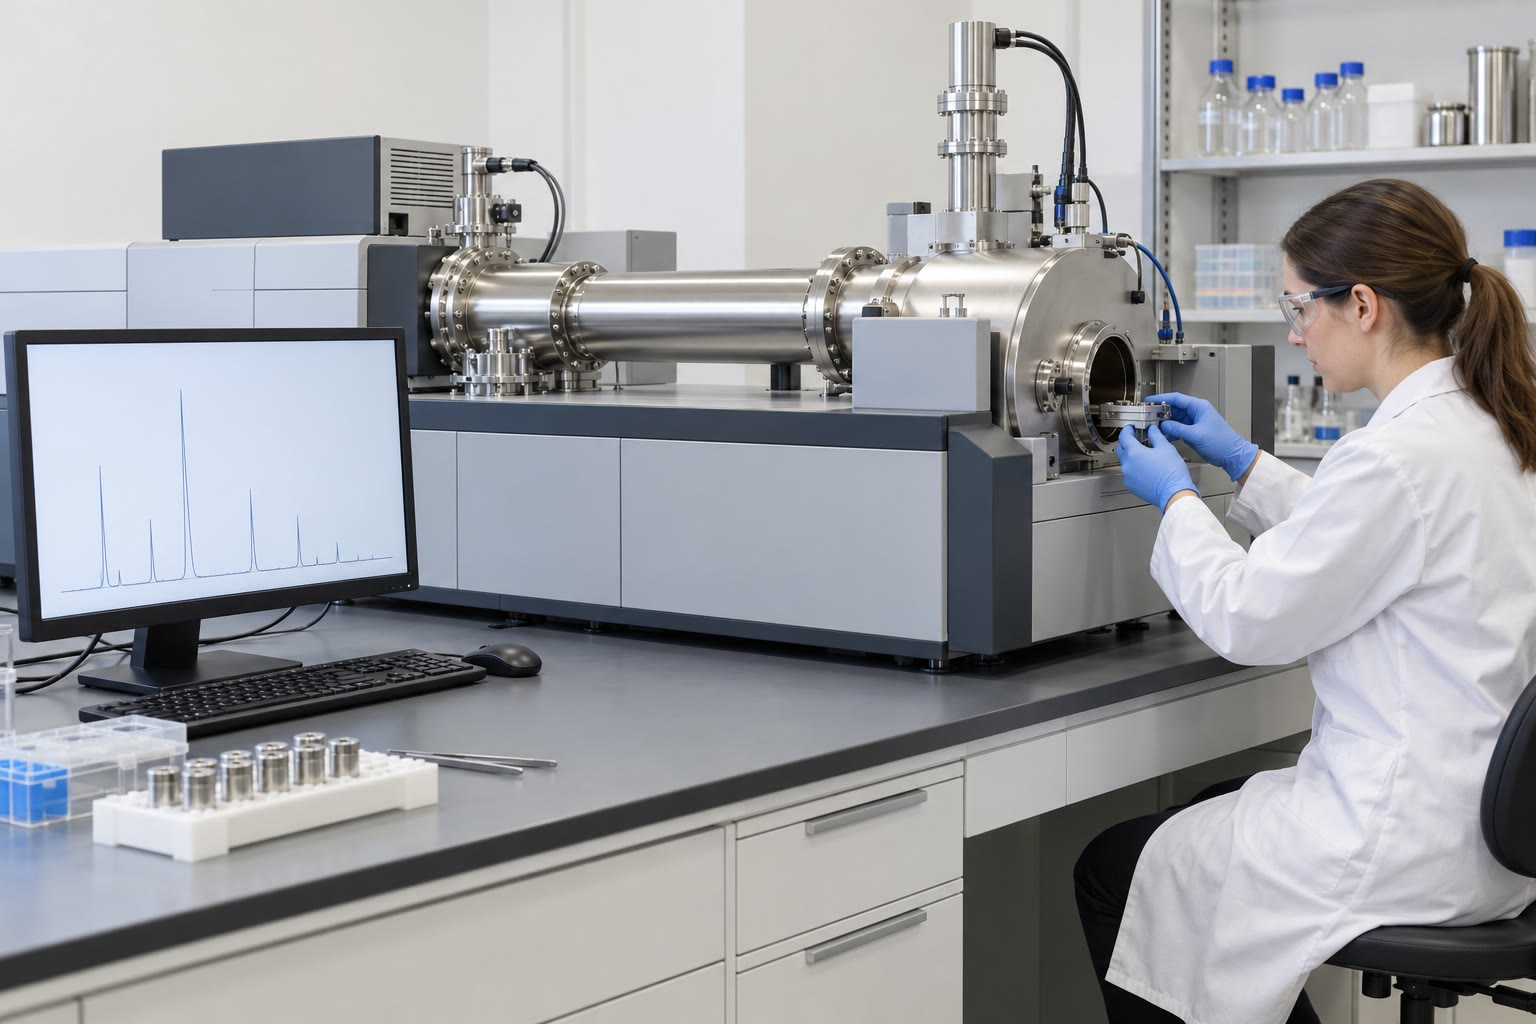
\includegraphics[width=0.66\linewidth]{images/book2/ai/g12-mass-spectrometer-lab.jpg}

{\small مطياف كتلة في مختبر: تُحمَّل عينة عند طرف
المصدر. رسم توضيحي مولَّد بالذكاء الاصطناعي.}
\end{omfigure}

والنسبة الابتدائية دليل أيضًا على مصدر الصهارة. فالروبيديوم
يفضّل المصهور حين ينصهر الوشاح، ولذلك تركّز على مر العصور
في \omterm{def:g12:continental-crust:continental-crust}{القشرة القارية}، التي صنعت تبعًا لذلك قدرًا أكبر من
السترونتيوم-87: فلصخور القشرة نسبة $^{87}\mathrm{Sr}/^{86}\mathrm{Sr}$ أعلى
من صخور الوشاح. والصهارة الناتجة عن انصهار القشرة ترث تلك النسبة العالية.
% ledger: tulane:radiometric

\section{عمر الأرض}

لا يعود أي صخر على الأرض إلى بداية الأرض: فأقدم صخر معروف،
نيس أكاستا، عمره 4.03 مليار سنة، وأقدم حبيبات الزركون 4.4
مليار. فقد انصهر السطح وتعرّى وأُعيد تدويره منذ ذلك الحين. أما تأريخ
الأرض نفسها فيأتي من النيازك، وهي شظايا من الأجسام الصغيرة
التي تكوّنت مع الكواكب، وظل بعضها أنظمة مغلقة
منذ ذلك الحين.
% ledger: bowring99:acasta, wilde01:zircon, usgs:age-earth (Book 1 row)

\begin{definition}[عمر الأرض]\label{def:g12:age-of-the-earth:age}
\emph{عمر الأرض}\index{عمر الأرض} هو الزمن المنقضي منذ
تكوّنت الأرض بتراكم أجسام أصغر، عند نشأة المجموعة
الشمسية. وهو، مقيسًا من النيازك بالتأريخ الإشعاعي،
\num{4.54} مليار سنة، بدقة واحد في المئة.
\end{definition}
% ledger: usgs:age-earth (Book 1 row)

في عام 1956 قاس كلير باترسون نظائر الرصاص في ثلاثة نيازك
حجرية ونيزكين حديديين. فنظيران من الرصاص يصنعهما
تفكك اليورانيوم، الرصاص-206 من اليورانيوم-238 والرصاص-207 من اليورانيوم-235،
بينما لا يصنع أي تفكك الرصاص-204. وكما في السترونتيوم، تقع نقاط النيازك
التي تكوّنت في الوقت نفسه على خط مستقيم، حين ترسم
$^{207}\mathrm{Pb}/^{204}\mathrm{Pb}$ بدلالة
$^{206}\mathrm{Pb}/^{204}\mathrm{Pb}$. ونيزك كانيون ديابلو الحديدي، في
أريزونا، لا يكاد يحوي يورانيوم: فرصاصه لم يتغير منذ تكوّن،
وهو يحدد الطرف السفلي من الخط، أي الرصاص الذي بدأت به المجموعة الشمسية.
% ledger: patterson56:table, patterson56:constants, usgs:age-earth (Book 1 row: Canyon Diablo troilite)

\begin{omfigure}
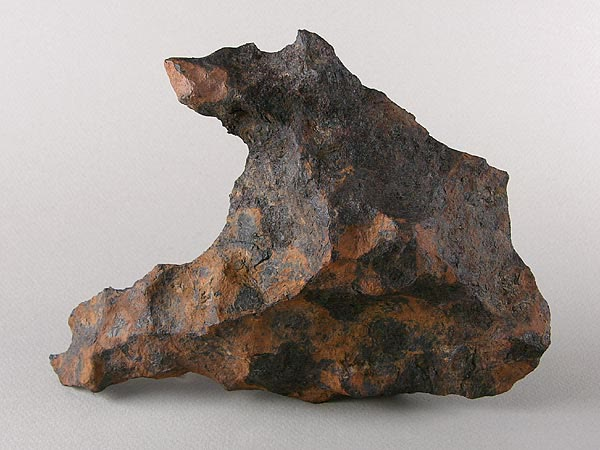
\includegraphics[height=4.2cm]{images/book2/g12-canyon-diablo-meteorite.jpg}

{\small شظية من نيزك كانيون ديابلو الحديدي، كتلتها \qty{2641}{g}.
الصورة: جيفري نوتكين، CC~BY-SA~2.5 (ويكيميديا كومنز).}
\end{omfigure}
% ledger: photo:g12-canyon-diablo

في الرصاص يتوقف الميل $m$ على العمر عبر نظيرَي اليورانيوم كليهما؛
ونُسلّم بالعلاقة هنا. وبالثوابت التي استعملها باترسون،
\[
  m = \frac{1}{137.8}\,\frac{e^{\lambda_{235}t}-1}{e^{\lambda_{238}t}-1},
  \qquad \lambda_{235} = \num{9.72e-10},\ \lambda_{238} = \num{1.537e-10}
  \text{ في السنة},
\]
وهذا يعطي:
\begin{center}
\small
\begin{tabular}{|l|c|c|c|c|c|c|}
\hline
العمر بمليارات السنين & 4.40 & 4.45 & 4.50 & 4.55 & 4.60 & 4.65 \\
الميل $m$ & 0.533 & 0.551 & 0.570 & 0.590 & 0.610 & 0.632 \\
\hline
\end{tabular}
\end{center}
% ledger: patterson56:constants
% values: pb_slope at 4.40-4.65 Ga (isochrons.py pb_slope)

\begin{omfigure}
\begin{tikzpicture}
\begin{axis}[omrecord, width=0.72\linewidth, height=6cm, xmin=0, xmax=56, ymin=0, ymax=40,
  xlabel={$^{206}\mathrm{Pb}/^{204}\mathrm{Pb}$}, ylabel={$^{207}\mathrm{Pb}/^{204}\mathrm{Pb}$}]
% computed in figdata/grade-12/isochrons.py; ledger: patterson56:table
\addplot[omDef, line width=0.9pt] table[x=x, y=y] {figdata/out/grade-12-isochrons-pbln.dat};
\addplot[omThm, only marks, mark=*, mark size=2pt] table[x=r206, y=r207, restrict expr to domain={\thisrow{idx}}{1:5}] {figdata/out/grade-12-isochrons-pbpb.dat};
\addplot[black, only marks, mark=o, mark size=2.6pt, line width=0.8pt] table[x=r206, y=r207, restrict expr to domain={\thisrow{idx}}{6:6}] {figdata/out/grade-12-isochrons-pbpb.dat};
\coordinate (nl) at (axis cs:50.28,34.86);
\coordinate (fc) at (axis cs:19.48,15.76);
\coordinate (cd) at (axis cs:9.5,10.36);
\coordinate (sed) at (axis cs:19.0,15.5);
\coordinate (sl) at (axis cs:30,25);
\end{axis}
\node[font=\scriptsize, anchor=north west] at ([xshift=2pt]nl) {نويفو لاريدو};
\node[font=\scriptsize, anchor=north west, align=left] at ([xshift=4pt, yshift=-2pt]fc) {فورست سيتي ومودوك\\الدائرة: رسوبيات محيطية};
\node[font=\scriptsize, anchor=north west, align=left] at ([xshift=3pt, yshift=-3pt]cd) {كانيون ديابلو وهنبري، حديديان};
\node[font=\scriptsize, text=omDef, anchor=south east] at (sl) {\foreignlanguage{arabic}{الميل 0.603: نحو 4.6 مليار سنة}};
\end{tikzpicture}

{\small \omterm{def:g12:age-of-the-earth:isochron}{خط تساوي العمر} بالرصاص عند باترسون: تقع النيازك الخمسة على خط واحد،
ويكاد يقع عليه أيضًا رصاص رسوبيات محيطية حديثة، تمثل الأرض.
المصدر: باترسون (1956)، الجدول~1.}
\end{omfigure}
% values: pb_slope 0.6026, pb_age_Ga 4.58, sediment_residual -0.39 (isochrons.py)

للخط المرسوم عبر النقاط الخمس ميل يبلغ نحو 0.603، بين
ميلَي 4.55 و4.60 مليار سنة في الجدول. وكانت نتيجة باترسون
نفسه، بعد حساب أخطاء القياسات وأخطاء ثوابت
التفكك، 4.55 مليار سنة، بزيادة أو نقصان 0.07. ثم قاس رصاص رسوبيات محيطية حديثة، تخلط
رصاصًا من كتلة عظيمة من قشرة الأرض: فوقعت على الخط نفسه. فقد
تطور رصاص الأرض كما تطور رصاص النيازك، على مدى الزمن نفسه: أي إن
الأرض في مثل عمرها.
% ledger: patterson56:table

وقد أكدت ذلك منذئذ مئات القياسات. فالنيازك تعطي أعمارًا
من 4.53 إلى 4.58 مليار سنة، وأقدم المواد الصلبة في المجموعة الشمسية،
وهي اشتمالات صغيرة غنية بالكالسيوم والألومنيوم توجد في بعض النيازك،
تكوّنت قبل \num{4567.30} مليون سنة، بزيادة أو نقصان 0.16. وقد تكوّنت الأرض
لاحقًا من مادة كهذه، ولهذا فعمرها، 4.54 مليار سنة، أقل
قليلًا من عمرها.
% ledger: usgs:age-earth (Book 1 row), connelly12:cai

\section{تمارين}

\begin{exercise}[$\star$]\label{exo:g12:age-of-the-earth:1}
أعطِ المصطلح: (أ) معدن لم تدخله ولم تخرج منه أي ذرة أم أو وليدة
منذ بدء ساعته؛ (ب) الخط المستقيم الذي تقع عليه معادن
متساوية العمر ومشتركة المصدر؛ (ج) الزمن المنقضي منذ تكوّنت الأرض
بالتراكم.
\end{exercise}

\begin{exercise}[$\star$]\label{exo:g12:age-of-the-earth:2}
مستعينًا بجدول غرانيت فاردن، رتّب عيناته الخمس بحسب
نسبة الروبيديوم-87 إلى السترونتيوم-86 فيها، من الأدنى. أيها يقع
أعلى على \omterm{def:g12:age-of-the-earth:isochron}{خط تساوي العمر}، ولماذا صنع أكبر قدر من السترونتيوم-87؟
\end{exercise}

\begin{exercise}[$\star$]\label{exo:g12:age-of-the-earth:3}
احسب عمر النصف للروبيديوم-87 من ثابت تفككه،
\num{1.3972e-11} في السنة. كم ضعفًا \omterm{def:g12:age-of-the-earth:age}{لعمر الأرض} يبلغ؟
\end{exercise}

\begin{exercise}[$\star$]\label{exo:g12:age-of-the-earth:4}
احسب $e^{\lambda t} - 1$ للروبيديوم-87 عند $t = 310$ مليون سنة
و$t = 480$ مليون سنة.
\end{exercise}

\begin{exercise}[$\star$]\label{exo:g12:age-of-the-earth:5}
رتّب بحسب التاريخ تقديرات فيليبس، وهولمز (1927)، وجولي، وكلفن
(1862)، وباترسون. كم ضعفًا للحد الأعلى من تقدير جولي
يبلغ \omterm{def:g12:age-of-the-earth:age}{عمر الأرض} المعتمد اليوم؟
\end{exercise}

\begin{exercise}[$\star\star$]\label{exo:g12:age-of-the-earth:6}
لمعدن من غرانيت فاردن (310 ملايين سنة، ونسبة ابتدائية 0.7080)
$^{87}\mathrm{Rb}/^{86}\mathrm{Sr} = 10.0$. ما نسبة
$^{87}\mathrm{Sr}/^{86}\mathrm{Sr}$ فيه اليوم؟ وكم كانت حين تكوّن
الغرانيت؟
\end{exercise}

\begin{exercise}[$\star\star$]\label{exo:g12:age-of-the-earth:7}
تعطي أربع عينات من شيست فاردن $(x, y)$ = \babelsublr{(0.90,~0.71806)}،
و\babelsublr{(2.60,~0.72950)}، و\babelsublr{(5.10,~0.74632)}، و\babelsublr{(9.40,~0.77525)}، حيث $x =
{}^{87}\mathrm{Rb}/^{86}\mathrm{Sr}$ و$y = {}^{87}\mathrm{Sr}/^{86}\mathrm{Sr}$.
(1) من العينتين الأولى والأخيرة، احسب الميل والعمر.
(2) تحقق من أن العينتين الوسطيين تقعان على الخط نفسه. (3) هل
النتيجة متسقة مع عمر الغرانيت البالغ 310 ملايين سنة ومع مبدأ
التقاطع؟
\end{exercise}

\begin{exercise}[$\star\star$]\label{exo:g12:age-of-the-earth:8}
لماذا لا يعطي صخر تتساوى نسبة الروبيديوم إلى السترونتيوم في جميع معادنه
أي خط تساوي عمر؟ ولماذا يحدد البيوتيت، في غرانيت فاردن،
الميل أفضل من سائر المعادن؟
\end{exercise}

\begin{exercise}[$\star\star$]\label{exo:g12:age-of-the-earth:9}
بعد تكوّن غرانيت فاردن بزمن طويل، جعل مائع ساخن البيوتيت فيه يفقد جزءًا
من السترونتيوم-87. (1) إلى أين تنتقل نقطته على مخطط \omterm{def:g12:age-of-the-earth:isochron}{خط تساوي العمر}؟
(2) ما العمر الذي يعطيه البيوتيت والبلاجيوكليز وحدهما حينئذ: أكبر من الحقيقي أم
أصغر؟ (3) كيف تكشف طريقة \omterm{def:g12:age-of-the-earth:isochron}{خط تساوي العمر} المشكلة؟
\end{exercise}

\begin{exercise}[$\star\star$]\label{exo:g12:age-of-the-earth:10}
(1) كم مرة يزيد \omterm{def:g12:age-of-the-earth:age}{عمر الأرض} على 96 مليون سنة التي قدّرها كلفن؟
(2) افترض جولي أن الأنهار تجلب الملح إلى البحر بمعدل
ثابت، وأن شيئًا منه لا يغادر البحر. أي هذين الافتراضين يجعل
عمره أقصر من الحقيقي إذا كان خاطئًا، ولماذا؟
\end{exercise}

\begin{exercise}[$\star\star$]\label{exo:g12:age-of-the-earth:11}
مستعينًا بقيم باترسون لكانيون ديابلو \babelsublr{(9.46,~10.34)} ونويفو لاريدو
\babelsublr{(50.28,~34.86)}، احسب ميل الخط المار بالنيزكين،
واقرأ العمر من جدول الميول.
\end{exercise}

\begin{exercise}[$\star\star\star$]\label{exo:g12:age-of-the-earth:12}
بازلت من منطقة فاردن، عمره أيضًا 310 ملايين سنة، نسبته
الابتدائية 0.7035، مقابل 0.7080 للغرانيت. (1) أي الصخرين أرجح
أن يأتي من وشاح منصهر، وأيهما من قشرة منصهرة؟ (2) فسّر
ذلك بما تعرفه عن الروبيديوم. (3) هل يمكن أن يكونا قد تبلورا من
صهارة واحدة؟
\end{exercise}

\begin{exercise}[$\star\star\star$]\label{exo:g12:age-of-the-earth:13}
(1) ما الكسر الباقي اليوم من الروبيديوم-87 الذي كان موجودًا حين تكوّنت
الأرض؟ ومن اليورانيوم-238 (عمر نصفه 4.47 مليار سنة)؟ (2) ما
ميل \omterm{def:g12:age-of-the-earth:isochron}{خط تساوي العمر} بالروبيديوم--السترونتيوم لصخر عمره مليون
سنة؟ ولماذا تُعد ساعة الروبيديوم--السترونتيوم ساعة رديئة للصخور الحديثة؟
\end{exercise}

\begin{exercise}[$\star\star\star$]\label{exo:g12:age-of-the-earth:14}
الخط المار بنيازك باترسون الخمسة هو $y = 4.438 + 0.6026\,x$.
(1) ما نسبة $^{207}\mathrm{Pb}/^{204}\mathrm{Pb}$ التي يتنبأ بها للرسوبيات
المحيطية، عند $x = 19.0$؟ قاس باترسون 15.5: فبأي نسبة مئوية
تختلفان؟ (2) ما العمر الذي يعطيه الميل 0.6026، من الجدول؟ قارنه بقيمة
باترسون $4.55 \pm 0.07$ مليار سنة.
\end{exercise}

\begin{exercise}[$\star\star\star$]\label{exo:g12:age-of-the-earth:15}
افترض كلفن أن كل الحرارة التي تفقدها الأرض، \qty{46.7}{TW} اليوم، حرارة
مختزنة. (1) يعوّض النشاط الإشعاعي نحو \qty{24.4}{TW} منها. بكم
يطيل ذلك وحده الزمن اللازم لفقد مخزون معين من الحرارة؟
(2) انطلاقًا من 96 مليون سنة، هل يكفي هذا لبلوغ العمر الحقيقي؟
(3) ما الذي فات كلفن وهو أهم من ذلك؟
\end{exercise}

\begin{problem}[{مسألة نهاية الأسبوع --- تأريخ غرانيت فاردن}]
\label{pb:g12:age-of-the-earth:1}
% exercise data from figdata/grade-12/isochrons.py; ledger: villa22:rb87, tulane:radiometric, ics:base.Carboniferous, ics:base.Permian
يقطع غرانيت تلال فاردن، المنطقة المتخيَّلة في هذه السلسلة،
الشيست المحيط به. وقد قاس مختبر خمسًا من عيناته (المثال أعلاه):
البلاجيوكليز \babelsublr{(0.35,~0.70952)}، والهورنبلند \babelsublr{(1.20,~0.71321)}،
والصخر الكلي \babelsublr{(3.10,~0.72146)}، وفلسبار البوتاسيوم \babelsublr{(6.40,~0.73578)}، والبيوتيت \babelsublr{(24.0,~0.81218)}، وكلٌّ منها في صورة
$(^{87}\mathrm{Rb}/^{86}\mathrm{Sr},\ ^{87}\mathrm{Sr}/^{86}\mathrm{Sr})$. وثابت
تفكك الروبيديوم-87 هو \num{1.3972e-11} في السنة.

\medskip
\noindent\textbf{الجزء الأول --- العينات.}
\begin{enumerate}
  \item أي العينات أغنى بالروبيديوم بالنسبة إلى السترونتيوم؟
  \item لماذا بدأت المعادن كلها بالنسبة نفسها
        $^{87}\mathrm{Sr}/^{86}\mathrm{Sr}$؟
  \item لماذا تؤخذ النسب إلى السترونتيوم-86؟
  \item أي النظائر الثلاثة ازداد منذ تكوّن الغرانيت، ولماذا؟
  \item كيف كانت تبدو النقاط الخمس على المخطط حين
        تكوّن الغرانيت لتوّه؟
\end{enumerate}

\medskip
\noindent\textbf{الجزء الثاني --- خط تساوي العمر.}
\begin{enumerate}[resume]
  \item احسب الميل عبر البلاجيوكليز والبيوتيت.
  \item احسب الميل عبر البلاجيوكليز والصخر الكلي.
  \item قارن الميلين. أيهما أوثق، ولماذا؟
  \item جد النقطة التي يلاقي فيها خط السؤال 6 المحور الرأسي.
  \item تحقق من أن فلسبار البوتاسيوم يقع على ذلك الخط.
\end{enumerate}

\medskip
\noindent\textbf{الجزء الثالث --- الميل والعمر.}
\begin{enumerate}[resume]
  \item اكتب العلاقة بين الميل و$e^{\lambda t}$.
  \item احسب $\lambda t$.
  \item احسب العمر $t$.
  \item أُرِّخ الشيست فكان عمره 480 مليون سنة. هل ترتيب
        العمرين هو ما تقتضيه العلاقات الحقلية؟
  \item يمتد الكربوني من 358.9 إلى 298.9 مليون سنة مضت. في
        أي عصر تكوّن الغرانيت؟
\end{enumerate}

\medskip
\noindent\textbf{الجزء الرابع --- النسبة الابتدائية والمصدر.}
\begin{enumerate}[resume]
  \item ماذا يمثل المقطع، 0.7080؟
  \item تكوّن بازلت من المنطقة بنسبة 0.7035. أي الصخرين
        نسبته الابتدائية أعلى؟
  \item لماذا تكون نسب صخور القشرة أعلى من نسب الوشاح؟
  \item ماذا توحي النسبة الابتدائية للغرانيت عن الصخر الذي
        انصهر فصنعه؟
  \item لخّص: كم عمر غرانيت فاردن؟
\end{enumerate}
\end{problem}
